% This must be in the first 5 lines to tell arXiv to use pdfLaTeX, which is strongly recommended.
\pdfoutput=1
% In particular, the hyperref package requires pdfLaTeX in order to break URLs across lines.

\documentclass[11pt]{article}

% Remove the "review" option to generate the final version.
\usepackage[final]{EMNLP2022}

% Standard package includes
\usepackage{times}
\usepackage{amsmath}
\usepackage{latexsym}
\usepackage{booktabs}       % professional-quality tables
\usepackage{multirow}
\usepackage{graphicx}
\usepackage{soul}
\usepackage{xcolor}
\usepackage{rotating}
\usepackage[framemethod=tikz]{mdframed}  % hot finding boxes
\usepackage{enumitem}


\newcommand{\ib}[1]{\textcolor{teal}{\small [IB: #1]}}
\newcommand{\jl}[1]{\textcolor{orange}{\small [JL: #1]}}
% For proper rendering and hyphenation of words containing Latin characters (including in bib files)
\usepackage[T1]{fontenc}
% For Vietnamese characters
% \usepackage[T5]{fontenc}
% See https://www.latex-project.org/help/documentation/encguide.pdf for other character sets

% This assumes your files are encoded as UTF8
\usepackage[utf8]{inputenc}
\usepackage{microtype}
\usepackage{hyperref}

\newcommand*\samethanks[1][\value{footnote}]{\footnotemark[#1]}
\newcommand{\todo}[1]{\textbf{\textcolor{red}{#1}}}

\newcommand{\new}[1]{{\color{red}\marginpar{\textcolor{red}{NEW}}{#1}}}

%%%%%%%%%%%%%%%%%%%%%%%%%%%%%%%%%%%%%%%%%%%%%%%%%%%%%%%%%%%%%%%%
% %%%%%%%%%% list of TODOs %%%%%%%%%%%%%%%%%%%%%%%%%%%%%%%%%%%%%
% 2.3: add details of gpt3 hyper params
% 
%%%%%%%%%%%%%%%%%%%%%%%%%%%%%%%%%%%%%%%%%%%%%%%%%%%%%%%%%%%%%%%%
\title{What Language Model to Train if You Have One Million GPU Hours?}

\author{\textbf{\underline{The BigScience Architecture \& Scaling Group}} \vspace{0.4cm}\\ \small
\textbf{Teven Le Scao}$^{1}$\thanks{~~Equal contribution.} \hspace{0.3cm}
\textbf{Thomas Wang}$^{1}$\samethanks \hspace{0.3cm}
\textbf{Daniel Hesslow}$^{2}$\samethanks \hspace{0.3cm}  \textbf{Lucile Saulnier}$^{1}$\samethanks \hspace{0.3cm}
\textbf{Stas Bekman}$^{1}$\samethanks \\
\small
\textbf{M Saiful Bari}$^3$ \hspace{0.3cm} \textbf{Stella Biderman}$^{4,5}$ \hspace{0.3cm} \textbf{Hady Elsahar}$^6$ \hspace{0.3cm} 
\textbf{Niklas Muennighoff}$^1$ \hspace{0.3cm} 
\textbf{Jason Phang}$^5$ \hspace{0.3cm} \textbf{Ofir Press}$^8$ \\
\small
\textbf{Colin Raffel}$^1$ \hspace{0.3cm}
\textbf{Victor Sanh}$^1$ \hspace{0.3cm}
 \textbf{Sheng Shen}$^9$ \hspace{0.3cm} \textbf{Lintang Sutawika}$^{10}$ \hspace{0.3cm} \textbf{Jaesung Tae}$^1$ \hspace{0.3cm} \textbf{Zheng Xin Yong}$^{11}$ \\
 \small
 \textbf{Julien Launay}$^{2, 12}$\thanks{~~Equal supervision.} \hspace{0.3cm}
 \textbf{Iz Beltagy}$^{13}$\samethanks\vspace{0.1cm} \\
 \small
 $^1$ Hugging Face \hspace{0.2cm} $^2$ LightOn \hspace{0.2cm} $^3$ NTU, Singapore \hspace{0.2cm} $^4$ Booz Allen \hspace{0.2cm} $^5$ EleutherAI \hspace{0.2cm} $^6$ Naver Labs Europe \hspace{0.2cm} $^7$ New York University\\
 \small$^8$ University of Washington \hspace{0.2cm} $^9$ Berkeley University \hspace{0.2cm} $^{10}$ Big Science \hspace{0.2cm} $^{11}$ Brown University \hspace{0.2cm} $^{12}$ LPENS \hspace{0.2cm} $^{13}$ Allen Institute for AI
}

\begin{document}
\onecolumn
\maketitle
\begin{abstract}
Transformer-based speech recognition models have achieved great success due to the self-attention (SA) mechanism that utilizes every frame in the feature extraction process.
Especially, SA heads in lower layers capture various phonetic characteristics by the query-key dot product, which is designed to compute the pairwise relationship between frames.
In this paper, we propose a variant of SA to extract more representative phonetic features.
The proposed phonetic self-attention (phSA) is composed of two different types of phonetic attention; one is similarity-based and the other is content-based.
In short, similarity-based attention captures the correlation between frames while content-based attention only considers each frame without being affected by other frames.
We identify which parts of the original dot product equation are related to two different attention patterns and improve each part with simple modifications.
Our experiments on phoneme classification and speech recognition show that replacing SA with phSA for lower layers improves the recognition performance without increasing the latency and the parameter size.

\end{abstract}
\section{Introduction}
\begin{figure}
    \centering
    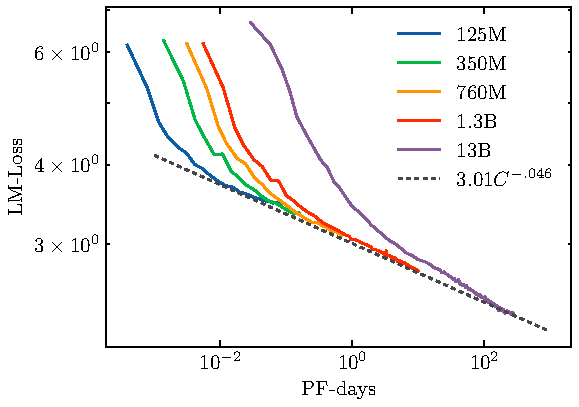
\includegraphics[width=\columnwidth]{figures/OscarScaling.pdf}
    \caption{\textbf{Smooth scaling of language modeling loss as compute budget and model size increase}. We observe a power-law coefficient $\alpha_C \sim 0.046$, in-line with \citet{kaplan2020scaling}. We use this fit to estimate the optimal size and number of tokens to train on for the final model given the available budget.}
    \label{fig:scaling}
\end{figure}

Recent years have seen the advent of large language models 
characterized by emergent capabilities (e.g., zero-shot generalization) arising from sheer scale alone~\cite{radford2019language,brown2020gpt3}.
Scaling LLMs results in a predictable increase in performance: simple scaling laws connect the number of parameters, pretraining dataset size, and compute budget~\cite{kaplan2020scaling,ganguli2022predictability,hoffmann2022training}, providing a clear path towards more capable models. This paradigm shift has been fueled by the wide~adoption of the Transformer~\cite{vaswani2017attention}, providing a scalable basis for practitioners to build upon. 

In this paper, we design an architecture and training setup for a multilingual 100B+ parameters model (BLOOM, \citet{bigscience_workshop_2022}), seeking to best use a fixed 1,000,000 A100-hours budget. Because of the costs involved with training large language models, we cannot exhaustively explore the landscape of possible models. Instead, we position ourselves as practitioners exploring "off-the-shelf" solutions. We thus test promising additions to the Transformer to attempt to reproduce their findings in a controlled, large-scale setting.

Although our main goal was to prepare the architecture and training setup of BLOOM, our findings are also valuable for practitioners building models in the 1-10B range, as they equally improve the performance of such smaller models. At variance with major works on large language models, we also make a significant effort towards reproducibility and openness: all of our pretrained models, code, and notes from our weekly meetings are made available. See Appendix \ref{sec:artefacts} for the relevant links.

\paragraph{Contributions.} We first study the impact of pretraining corpora, positional embeddings, activation functions, and embedding norm on zero-shot generalization. We base our study on the popular GPT-2 architecture \cite{radford2019language}, with experiments at the 1.3B parameters scale. We then consider the impact of massive multilinguality, showing language-specific scaling laws in a multilingual setting for the first time. Finally, we describe our approach to drafting an architecture for the final 176B parameters BLOOM model.



\section{Methods}

\begin{table*}[t]
\begin{center}
\begin{tabular}{@{}lccccc@{}}
\toprule
\multicolumn{1}{c}{\textbf{Model}} & \textbf{Parameters}            & \multicolumn{4}{c}{\textbf{Pretraining tokens}}                                                                       \\ \midrule
                                               & \multicolumn{1}{l}{}  & \multicolumn{1}{l}{Dataset} & \multicolumn{1}{l}{112B} & \multicolumn{1}{l}{250B} & \multicolumn{1}{l}{300B} \\ \midrule
\textbf{OpenAI} --- Curie          & 6.7B            & \multicolumn{1}{l}{}        &                          &                          & \underline{49.28}           \\
\textbf{OpenAI} --- Babbage          & 1.3B            & \multicolumn{1}{l}{}        &                          &                          & \textbf{45.30}        \\
\textbf{EleutherAI} --- GPT-Neo              & 1.3B                  & The Pile                    &                          &                          & 42.94                    \\ \midrule
\multirow{1}{*}{\textbf{Ours}}                             & 13B                   & OSCAR v1                      &                          &                          & 47.09                    \\ \midrule
    \multirow{3}{*}{\textbf{Ours}}                                                        & 1.3B & The Pile                    & \textbf{42.79}                    & 43.12                    & 43.46                    \\
                                                           & 1.3B & C4                          & 42.77                    &                          &                          \\
                                                           & 1.3B & OSCAR v1                       & 41.72           &                          &                          \\ \bottomrule
\end{tabular}
\end{center}
\caption{\textbf{Pretraining datasets with diverse cross-domain high-quality data improves zero-shot generalization.} Average accuracy on EAI harness (higher is better) using different pretraining corpora and comparison with baseline models. \textbf{Bold is best 1.3B model for amount of tokens seen}, \underline{underline is best overall}.}
\label{tab:validation}
\end{table*}

We first justify our choice to base our model on the popular recipe of combining a decoder-only model with an autoregressive language modeling objective, and introduce our experimental setup. We then discuss our evaluation benchmarks, and motivate our choice of zero-shot generalization as our key metric. Finally, we introduce the baselines we compare to throughout the paper.

\subsection{Architecture and Pretraining Objective}
\label{sec:t5x}

In this paper, we base all models on a decoder-only Transformer pretrained with an autoregressive language modeling objective. This is a popular choice for large language models \cite{brown2020gpt3, rae2021scaling, thoppilan2022lamda}, possibly because it lends itself to zero-shot application to many downstream tasks \cite{radford2019language}. Alternatives include encoder-decoder models trained with a span-corruption objective (e.g., T5~\citet{raffel2019t5}), as well as non-causal decoders models with visibility over a prefix (so-called Prefix LMs, \citet{liu2018generating, dong2019unified}).   

Our decision is motivated by the findings of~\citet{wang2022language}, which showed that decoder-only models combined with an autoregressive language modeling objective provide the best zero-shot generalization abilities immediately after pretraining. Although multitask finetuning~\cite{Sanh2021MultitaskPT,wei2021finetuned} will instead favor an encoder-decoder with span corruption for best zero-shot generalization, \citet{wang2022language} found a compromise between these two practices. Following autoregressive pretraining, decoder-only models can be efficiently adapted into non-causal decoders, simply by extending pretraining with span corruption. This adaptation produces a second model, which can provide excellent zero-shot generalization after multitask finetuning. Accordingly, we follow their recommendation, and train an autoregressive decoder-only model first which we will later consider adapting and finetuning. 

\subsection{Experimental Setup} 
We follow the architectures GPT-2~\citep{radford2019language} and the hyperparameters of GPT-3 \citep{brown2020gpt3}. For learning rate, we use a maximum value of $2 \times 10^{-4}$, with a linear warm-up over 375M tokens, followed by cosine decay to a minimum value of $1 \times 10^{-5}$. We use a 1M tokens batch size, with linear ramp-up over the first 4B tokens, and a sequence length of 2,048. We use the Adam optimizer \cite{kingma2014adam}, with $\beta_1=0.9$, $\beta_2=0.999$, $\epsilon=1 \times 10^{-8}$, weight decay 0.1, and gradient clipping to 1.0. We also tie the word embedding and softmax matrix~\citep{tying}. Unless noted otherwise, we conduct our experiments with 1.3B parameters models, pretraining on 112B tokens. 

We picked this size and dataset size as a compromise between compute cost and the likelihood that our conclusions would transfer to the target 100B+ model. Notably, we needed to be able to reliably measure zero-shot generalization above random chance. We note that training for 112B tokens 1.3B parameters models bring them significantly above the optimality threshold of~\citet{kaplan2020scaling}, and of~\citet{hoffmann2022training}. 


The main architectural difference with GPT-3 is that all our layers use full attention, while GPT-3 uses alternating sparse attention layers~\citep{sparse}. 
The main value of sparse attention layers is to save compute with long sequence lengths. However, at the 100B+ scale, sparse attention layers
provide negligible compute savings, as the vast majority of the compute is spent on the large feed-forward layers.
\citet{kaplan2020scaling} estimated the amount of compute per token to be:
\begin{equation*}
C_\text{forward} = 2 \times (12 n_\text{layer} d^2 + n_\text{layer} n_\text{ctx} d),
\end{equation*}
where $C_\text{forward}$ is the cost for the forward pass, $n_\text{layer}$ is the number of layers, $d$ is the hidden dimension, and $n_\text{ctx}$ is the sequence length. This means if $12 d >> n_\text{ctx}$, the 
second $n_\text{layer} n_\text{ctx} d$ term is negligible, which is the case for our final model 
where $d > 10,000$ and $n_\text{ctx} = 2048$. 

\paragraph{What is a FLOP exactly?} We report throughput per GPU in FLOPS and total budgets in PF-days (i.e. one PFLOPS sustained for a day). It is important to highlight that FLOPS are never directly measured, but always estimated, with widely different practices across papers. We refer to \emph{model} FLOP the estimates based on the $C=6ND$ formula from \citet{kaplan2020scaling}, where $C$ is the total compute, $N$ the model size, and $D$ the number of tokens processed. These are the FLOP actually used to train the model, and which are used for scaling laws. We refer to \emph{hardware} FLOP the estimates reported by our codebase, using the formula from \citet{narayanan2021efficient}. This notably includes gradient checkpointing, which trades additionnal computations for reduced memory needs, and a more thorough accounting of operations.

\subsection{Evaluation Benchmarks} 
We measure upstream performance using the language modeling loss on an held out sample of the pretraining dataset. However, it is not always possible to compare losses across objectives and tokenizers. Moreover, as upstream performance is not always aligned with task performance \cite{Tay2021ScaleEI}, we must also measure downstream performance explicitly. We could use zero/few-shot generalization, with or without specific finetuning. 

Specifically, we choose to measure zero-shot generalization on a diverse set of tasks. Few-shot and zero-shot results are strongly correlated: we found a Pearson correlation coefficient of 0.93 between zero-shot and few-shot performance across model sizes in \citet{brown2020gpt3}. We do not rely on finetuning as it is not how the main final model is likely to be used, given its size and the challenges associated with finetuning at the 100B+ scale. 

We use the popular EleutherAI Language Model Evaluation Harness (EAI harness, \citet{eval-harness}), evaluating models across 27 diverse tasks that are similar to those used in~\citet{brown2020gpt3} (see Appendix \ref{sec:sup_eval} for a list of tasks). Overall, the random baseline on our benchmark sits at 33.3\%. 

\subsection{Baselines} 
We use GPT-Neo~\cite{gpt-neo}, a~1.3B decoder-only autoregressive language model trained on the Pile~\cite{gao2020pile}, and GPT-3~\cite{brown2020gpt3}, accessed via the OpenAI API. We evaluate two models, Babbage and Curie\footnote{These models are now referred to as \texttt{text-babbage-001} and \texttt{text-curie-001}.}. Based on \citet{gaosize} and our own analysis, we assume  
Babbage is 1.3B while Curie is 6.7B based on how close our computed results are to those reported in the original paper. However, as details of the OpenAI API are kept secret, there is no way to make sure that the models are actually the ones described in~\citet{brown2020gpt3} -- the number of pretraining tokens reported in Table \ref{tab:validation} is thus to be taken cautiously.
\section{Impact of Pretraining Data}


\begin{table*}[t]
  \begin{center}
    \begin{small}
      \begin{tabular}{l|l}
        \toprule
        \textbf{Original Persona} & \textbf{Revised Persona}\\
        \midrule
I love the beach. & To me, there is nothing like a day at the seashore. \\
My dad has a car dealership & My father sales vehicles for a living. \\
I just got my nails done & I love to pamper myself on a regular basis. \\
I am on a diet now & I need to lose weight. \\
Horses are my favorite animal. &  I am into equestrian sports. \\
\midrule
\ifarxiv
I am an eccentric hair stylist for dogs & I work with animals. \\ %', 'I am a quirky dog groomer ']
My favorite past time is collecting Civil War antiques. & I like finding or buying historical artifacts. \\
I fake a British accent to seem more attractive. & I heard girls liked foreigners.\\
I have been married four times and widowed three. & I have a lot of experience with marriage\\
I have an allergy to mangoes & I have reactions to certain fruits. \\
\midrule
\fi
I play a lot of fantasy videogames. & RPGs are my favorite genre. \\
I have a computer science degree. & I also went to school to work with technology. \\
My mother is a medical doctor & The woman who gave birth to me is a physician. \\
I am very shy. & I am not a social person.\\
I like to build model spaceships.& I enjoy working with my hands. \\
\bottomrule
      \end{tabular}
      \caption{Example Personas (left) and their revised versions (right) from the {\sc persona-chat} dataset.
The revised versions are designed to be characteristics that the same persona might have, which could be rephrases, 
generalizations or specializations.
 \label{table:persona-examples}}
    \end{small}
  \end{center}
\end{table*}


\begin{table*}[t]
  \begin{center}
    \begin{small}
      \begin{tabular}{l|l}
        \toprule
        \textbf{Persona 1} & \textbf{Persona 2}\\
        \midrule
I like to ski & I am an artist\\
My wife does not like me anymore & I have four children\\
I have went to Mexico 4 times this year & I recently got a cat \\
I hate Mexican food &  I enjoy walking for exercise \\
I like to eat cheetos &  I love watching Game of Thrones\\
\bottomrule
\multicolumn{2}{l}{ }\\
\multicolumn{2}{l}{[PERSON 1:] Hi}\\
\multicolumn{2}{l}{[PERSON 2:] Hello ! How are you today ?}\\
\multicolumn{2}{l}{[PERSON 1:] I am good thank you , how are you.}\\
\multicolumn{2}{l}{[PERSON 2:] Great, thanks ! My children and I were just about to watch Game of Thrones. }\\
\multicolumn{2}{l}{[PERSON 1:] Nice ! How old are your children?}\\
\multicolumn{2}{l}{[PERSON 2:] I have four that range in age from 10 to 21. You?}\\
\multicolumn{2}{l}{[PERSON 1:] I do not have children at the moment.}\\ 
\multicolumn{2}{l}{[PERSON 2:] That just means you get to keep all the popcorn for yourself.}\\
\multicolumn{2}{l}{[PERSON 1:] And Cheetos at the moment!}\\
\multicolumn{2}{l}{[PERSON 2:] Good choice. Do you watch Game of Thrones?}\\
\multicolumn{2}{l}{[PERSON 1:] No, I do not have much time for TV.}\\
\multicolumn{2}{l}{[PERSON 2:] I usually spend my time painting: but, I love the show.}\\
      \end{tabular}
      \caption{Example dialog from the {\sc persona-chat} dataset. Person 1 is given their own persona (top left) at the beginning of the chat, but does not know the persona of Person 2, and vice-versa. They have to get to know each other during the conversation.
 \label{table:persona-chat-example}}
    \end{small}
  \end{center}
\end{table*}



\section{The {\sc persona-chat} Dataset} 

The aim of this work is to facilitate more engaging and more personal chit-chat dialogue. The {\sc persona-chat} dataset is a crowd-sourced dataset, collected via Amazon Mechanical Turk, where each of the pair of speakers condition their dialogue on a given profile, which is provided. 
%The dataset and its corresponding data collection source  code, as well as models trained on the data, are all available open source in ParlAI\footnote{\small{\url{http://parl.ai}}}).

The data collection consists of three stages:

%\begin{itemize}

%\item
(i) Personas: we crowdsource a set of 1155 possible personas, each consisting of at least 5 profile sentences, setting aside 100 never seen before personas for validation, and 100 for test.

%\item
(ii) Revised personas: to avoid modeling that takes advantage of trivial word overlap, we crowdsource  additional rewritten sets of the same 1155 personas, with related sentences that are rephrases, generalizations or specializations, rendering the task much more challenging.

(iii) Persona chat: we pair two Turkers and assign them each a random (original) persona from the pool, and ask them to chat. This resulted in a dataset of 162,064 utterances over 10,907 dialogs, 15,602 utterances (1000 dialogs) of which are set aside for validation, and 15,024 utterances
(968 dialogs) for test.

%\end{itemize}

The final dataset and its corresponding data collection source  code, as well as models trained on the data, are all available open source in ParlAI\footnote{ {\small{\url{http://parl.ai}}}}.
%\small\url{https://github.com/facebookresearch/ParlAI/tree/master/projects/personachat}}.


In the following, we describe each data collection stage and the resulting tasks in more detail.

%The final dataset is available in ParlAI\footnote{\url{https://github.com/facebookresearch/ParlAI/tree/master/parlai/tasks/personachat}}. In the following, we describe each data collection stage in more detail.
%The final dataset will be made publicly available.


\if 0
With this resource, we then consider two tasks which measure the ability of models to engage their dialogue partner in personal conversation:
\begin{itemize}
\item Task 1: Next utterance prediction. Given a dialogue history, predict the next thing to say.  %This can be either conditioned on a profile or 
%One can consider this task either with or without conditioning on known profiles.
\item Task 2: Profile prediction. Given a dialogue history, predict the other speaker's profile.
\end{itemize}

In the following, we describe each data collection stage and the resulting tasks in more detail.
\fi 





\subsection{Personas}

We asked the crowdsourced workers to create a character (persona) description using 5 sentences, providing them only a single example:

{\em ``I am a vegetarian. I like swimming.  My father used to work for Ford.  My favorite band is Maroon5. I got a new job last month, which is about advertising design.''}

Our aim was to create profiles that are natural and descriptive, and contain typical topics of human interest that the speaker 
can bring up in conversation. Because the personas are not the real profiles of the Turkers,
  the dataset does not contain personal information (and they are told specifically not to use any).
We asked the workers to make each sentence short, with a maximum of 15 words per sentence.
This is advantageous both for humans and machines: if they are too long, crowdsourced workers are likely to lose interest, and for machines the task could become more difficult.

Some examples of the  personas collected are given in Table \ref{table:persona-examples} (left).

\subsection{Revised Personas}

A difficulty when constructing dialogue datasets, or text datasets in general, is that in order to
encourage research progress, the task must be carefully constructed so that is neither too
 easy nor too difficult for the current technology 
 \citep{voorhees1999trec}.
One issue with conditioning on textual personas is that there is a danger that humans will, even if asked not to,
unwittingly repeat profile information either verbatim or with significant word overlap.
This may make any subsequent machine learning tasks less challenging, and the solutions will not generalize to
more difficult tasks. This has been a problem in some recent datasets:
for example, the dataset curation technique used for the well-known SQuAD dataset
suffers from this word overlap problem to a certain extent \citep{chen2017reading}.

To alleviate this problem, we presented the original personas we collected to a new set of crowdworkers
and asked them to rewrite the sentences so that a new sentence is about 
{\em ``a related characteristic that the same person may have''},
hence the revisions could be rephrases, generalizations or specializations.
For example {\em ``I like basketball''} can be revised as {\em ``I am a big fan of Michael Jordan''}
not because they mean the same thing but because the same persona could contain both. 

In the revision task, workers are instructed not to trivially rephrase the sentence by copying the original words.
However, during the entry stage if a non-stop word is copied we issue a
warning, and ask them to rephrase, guaranteeing that the instructions are followed. 
For example, {\em ``My father worked for Ford.''} can be revised to
{\em ``My dad worked in the car industry''}, but not
{\em ``My dad was employed by Ford.''} due to word overlap.

\ifarxiv
Finally, we encourage the construction of  natural sentences. In earlier versions of the task we noticed that
the word overlap constraint caused unwanted unnatural constructions such as {\em ``I like eating pretzels''} revised as
{\em ``I like to chew and swallow twisted bread with salt''}. Giving explicit instructions about this seemed to help,
where we prefer a revision like {\em ``I enjoy beers and beer snacks''}.
\fi

Some examples of the revised personas collected are given in Table \ref{table:persona-examples} (right).


\subsection{Persona Chat}\label{personachatter}

After collecting personas, we then collected the dialogues themselves, conditioned on the personas.
For each dialogue, we paired two random crowdworkers, and gave them the instruction that they will chit-chat with another worker, while
playing the part of a given character. We then provide them with a randomly chosen persona from our pool, different to their partners.
The instructions are on purpose quite terse and simply ask them to 
``chat with the other person naturally and try to get to know each other''.
In an early study we noticed the crowdworkers tending to talk about themselves (their own persona) too much, so
we also added the instructions
``both ask questions and answer questions of your chat partner'' which seemed to help.
We also gave a bonus for high quality dialogs.
The dialog is turn-based, with a maximum of 15 words per message.
We again gave instructions to not  trivially copy the character descriptions into the messages,
but also wrote explicit code sending them an error if they tried to do so, using simple string matching.
We define a minimum dialogue length which is randomly between 6 and 8 turns each for each dialogue.
An example dialogue from the dataset is given in Table  \ref{table:persona-chat-example}.


\subsection{Evaluation}

We focus on the standard dialogue task of predicting the next utterance given the dialogue history, but consider this task both with and without the profile information being given to the learning agent. Our goal is to enable interesting directions for future research, where chatbots can for instance have personalities, or imputed personas could be used to make dialogue more engaging to the user.

We consider this in four possible scenarios: conditioning on no persona, your own persona, their persona, or both. These scenarios can be tried using either the original personas, or the revised ones.
We then evaluate the task using three metrics: (i) the log likelihood of the correct sequence, measured via perplexity, (ii) F1 score, and (iii) 
next utterance classification loss, following \newcite{lowe2015ubuntu}.
%Next utterance classification loss 
The latter consists of choosing $N$ random distractor responses from other dialogues (in our setting, $N$=19) and the model selecting the best response among them, resulting in a score of one if the model chooses the correct response, and zero otherwise (called hits@1 in the experiments). %Its main advantage is that it is easy to interpret.

\if 0
As dialogue has many possible responses, leading to a multi-modal distribution of words, word overlap measures do not work well as evaluation metrics \citep{liu2016not,serban2015survey}.
While word level perplexity has many deficiencies as a measure of conversational success, it is standard in more general language modeling, 
and can still capture multi-modal distributions to a certain extent as 
good response word choices should still have high probability.
Thus we include it here.
\fi

\if 0 
\subsection{Persona-Chat Tasks}

The goal of our tasks is to facilitate more engaging and more personal chit-chat dialogue. Our setting naturally leads to two tasks: predicting the next utterance, and predicting the profile of the interlocutor. Both tasks enable interesting directions for future research, where chatbots can for instance have personalities, or imputed personas could be used to make dialogue more engaging to the user. In what follows, we describe the tasks in more detail.

\subsubsection{Next Utterance Prediction}

In the first task, the goal is, given the previous dialogue history and optionally persona information, to generate the response (the next utterance). We thus consider this in four possible scenarios: conditioning on no person, your own persona, their person, or both. We can also try each of these scenarios using either the original personas, or the revised ones.

We evaluate this task using two metrics: (i) the log likelihood of the correct sequence, measured via perplexity and (ii) 
next utterance classification loss, following \cite{lowe2015ubuntu}.

Perplexity is an appealing metric for dialogue as there are many possible responses, leading to a multi-modal distribution of words, which it can still capture as good response word choices should still have high probability. Next utterance classification loss consists of choosing $N$ random distractor responses from other dialogues (in our setting, $N$=19) and choosing the best among them, resulting in a score of one if the model chooses the correct response, and zero otherwise. Its main advantage is that it is easy to interpret.

\subsubsection{Profile Prediction}

In the second task, the goal is, given the agent's own persona and the entire dialogue history as input, to predict the other speaker's persona.

We use the same metrics for evaluating this setting by considering each entry in the other speaker's profile independently as a separate label. We can again consider the evaluation in two settings: using the original personas, or the revised ones. 
\fi


\section{Architecture Ablations}
We now consider ablation studies to better identify the best positional embedding, activation function, and embedding normalization placement. 

\subsection{Positional Embeddings}

\begin{table}[b]
\begin{center}
\begin{tabular}{@{}cc@{}}
\toprule
\textbf{Positional Embedding} & \textbf{Average EAI Results}\\
\midrule
None & 41.23\\
Learned & 41.71\\
Rotary & 41.46\\
ALiBi & \textbf{43.70} \\ 
\bottomrule
\end{tabular}
\end{center}
\caption{\textbf{ALiBi significantly outperforms other embeddings for zero-shot generalization.} All models are trained on the OSCAR dataset for 112 billion tokens.}
\label{tab:positional}
\end{table}

\paragraph{Background} Originally, both static sinusoidal position embeddings and learned position embeddings were proposed to capture positionnal information; the latter are popular in large language models \cite{brown2020gpt3}. 
\citet{su2021roformer} proposed rotary embeddings, where the query and key representations inside the self-attention mechanism are modified such that the attention captures relative distances between them. Recently, \citet{press2021alibi} introduced a method which does not use embeddings, instead directly attenuating the attention scores based on how far away the keys/queries are. 

\paragraph{Results} We compare learned, rotary, and ALiBi position embeddings, and include a baseline without position embeddings. Our results are presented in Table~\ref{tab:positional}. Although learned positional embeddings outperform rotary embeddings, ALiBi yields significantly better results than all alternatives. We also confirm the findings of~\citet{biderman2021nopos}: a baseline with no positional information exhibits competitive performance. While bidirectional models require positional embeddings to determine the location of tokens, we find autoregressive models can simply leverage the causal attention mask. We also confirm the ability of ALiBi to extrapolate to longer sequences than trained on in Figure \ref{fig:extrapolation}. Note that results in Table~\ref{tab:positional} do not use any extrapolation: ALiBi embeddings are a better choice even without taking into account their ability to extrapolate. 

\begin{figure}[h]
    \centering
    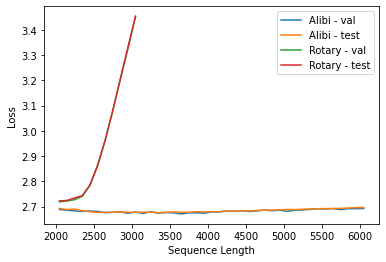
\includegraphics[width=\columnwidth]{figures/extrapolation.png}
    \caption{\textbf{ALiBi embeddings can effectively extrapolate past the sequence length on which the model was trained, while rotary embeddings can not.} This is in line with the findings of \citet{press2021alibi}.}
    \label{fig:extrapolation}
\end{figure}

\begin{table}[b]
\begin{center}
\begin{tabular}{@{}cc@{}}
\toprule
\textbf{Activation function} & \textbf{Average EAI Results}\\
\midrule
GELU & 42.79\\
SwiGLU & \textbf{42.95}\\
\bottomrule
\end{tabular}
\end{center}
\caption{\textbf{SwiGLU slightly outperforms GELU for zero-shot generalization.} Models trained on The Pile for 112 billion tokens.}
\label{tab:activation}
\end{table}

\begin{mdframed}
\textbf{Finding 2.} ALiBi positional embeddings significantly outperforms other embeddings for zero-shot generalization.
\end{mdframed}


\subsection{Activation Functions}

\paragraph{Background.} Large language models by and large still mostly use the GELU activation \cite{hendrycks2016gaussian}. We evaluate a recently proposed alternative, SwiGLU \cite{shazeer2020swiglu}, which combines both Gated Linear Units \cite{dauphin2016glu} with the Swish activation function \cite{ramachandran2017searching}. 

SwiGLU uses $50\% $ extra parameters in the feed-forward layers. As suggested in \citet{shazeer2020swiglu}, we compensate for this by reducing the hidden size of the feed-forward layer. 

\paragraph{Results.} We present our results in Table~\ref{tab:activation}. SwiGLU produces slightly better results than GELU. For our final model, we adopted GELU, as we initially observed a lower throughput for SwiGLU. However, further benchmarking identified that this overhead was primarily associated with the change in the hidden size of the feedforward network. Indeed, this new size, 5,456, is divisible by neither the warp size of the GPU~\citep{Lashgar2013WarpSI} nor the number of streaming multiprocessors, resulting in both tile and wave quantization. We accordingly recommend using SwiGLU for future models.


\subsection{Embedding Norm}

\citet{bitsandbytes} suggests that greater stability of training can be achieved by including an extra layer normalization \cite{layernorm} after the embedding layer. We evaluate the performance impact of such a modification in Table~\ref{tab:emb_norm}. We note that this incurs a significant reduction in the performance of the model. However, models above 100 billion parameters are notoriously unstable and require considerable engineering efforts in order to be kept stable. If this addition provides increased stability when training, it may be valuable. 


\begin{table}[b]
\begin{center}
\begin{tabular}{@{}cc@{}}
\toprule
\textbf{Embedding Norm} & \textbf{Average EAI Results}\\
\midrule
No & \textbf{43.46}\\
Yes &  42.24\\
\bottomrule
\end{tabular}
\end{center}
\caption{\textbf{Layer normalization after the embedding layer diminishes performance significantly.} Models trained on The Pile for 300 billion tokens.}
\label{tab:emb_norm}
\end{table}

\begin{mdframed}
\textbf{Finding 3.} Adding layer normalization after the embedding layer incurs a significant penalty on zero-shot generalization. 
\end{mdframed}


\begin{table*}[t!]
\begin{center}
% \setlength{\tabcolsep}{5pt}F
\begin{tabular}{@{}rc|cccccccc|c@{}}
\toprule
\textbf{Model} &  \textbf{Size} & EN & ZH & ES & FR & VI & AR & HI & UR & \textbf{Average} \\
\midrule
XGLM~(\citeauthor{XGLM}) & 7.5B & 54.5 & 45 & 38.2 & 50.7 & 47.5 & 47.5 & 43.4 & 42.7 & 46.19 \\
XGLM (reprod.)  & 7.5B & 53.85 & 45.21 & 41.7 & 49.82 & 47.35 & 46.37 & 43.19 & 42.3 & 46.22 \\
XGLM  & 1.7B & 49.68 & 44.63 & 37.39 & 47.94 & 42.75 & 45.65 & 44.35 & 43.19 & 44.45 \\
Ours  & 1.3B & 49.9 & 44.53 & 36.77 & 46.51 & 45.75 & 43.41 & 45.95 & 42.91 & 44.47\\
\bottomrule
\end{tabular}
\end{center}
\caption{\textbf{Our multilingual 1.3B model achieves accuracy on zero-shot XNLI in line with XGLM~\citet{XGLM}.} First row is the reported XGLM results, and the second is our reproduction of their results to validate our multilingual evaluation setup. Last two rows show that our multilingual model matches the XGLM results. } 
\label{tab:mutlilingual_xnli}
\end{table*}

\section{Multilinguality}
\begin{table}[b]
\begin{center}
\begin{tabular}{@{}cc@{}}
\toprule
\textbf{Pretraining} & \textbf{Average EAI Results}\\
\midrule
English-only  & \textbf{41.72}\\
Multilingual  & 38.55\\
\bottomrule
\end{tabular}
\end{center}
\caption{\textbf{Multilingual pretraining very significantly diminishes English zero-shot generalization.} Both models trained on OSCAR for 112B tokens.}
\label{tab:mutlilingual}
\end{table}




The majority of 100B+ language models have been trained in English, with notable exceptions in Chinese~\citep{zeng2021pangu, wu2021yuan} and Korean~\cite{Kim2021WhatCC} models. Smaller massively multilingual models have seen wider adoption \cite{mT5}, but these models are not suitable for zero-shot. Recent results on large GPT-like multilingual models show that English-only performance is usually disappointing \cite{XGLM}. 

\paragraph{Training data.}
We train a multilingual model to evaluate the effectiveness and potential impacts of this practice. 
We use the OSCAR dataset~\citep{ortiz2019oscar}, but here we include multiple languages, not only English as in the earlier experiments. 
The languages we include are Arabic, Basque, Bengali, Chinese, Catalan, English, French, Hindi, Indonesian, Portuguese, Spanish, Urdu, and Vietnamese.
We sample each language with a different probability that downsamples the most frequent languages 
and upsamples the least frequent ones, so that all languages 
are represented. We estimate the sampling probabilities similar to~\citet{Xue2021mT5AM}.




\paragraph{English-only evaluation.}
We first evaluate our multilingual model on the same set of English benchmarks we have used previously, in Table~\ref{tab:mutlilingual}. Multilinguality significantly lowers accuracy on the English benchmark, which is in line with the results from~\citet{XGLM}. 

\paragraph{Multilingual evaluation.}
Zero-shot multilingual evaluation is more challenging to setup because it requires writing new prompts for each new language. Therefore, instead of manually writing prompts for each language, we follow the strategy proposed by~\citet{XGLM}, using English prompts for non-English examples--this can be viewed as cross-lingual zero-shot generalization. They validated this strategy by demonstrating its ability to achieve zero-shot performance on par with (and sometimes even better than) human-written language-specific prompts. This strategy also demonstrates cross-lingual abilities.

\definecolor{shadecolor}{rgb}{0.93,0.93,0.93}


We evaluate on XNLI~\citep{conneau2018xnli}, a multilingual NLI dataset  that covers 8 of the languages we use for training. 
%The task uses the following English cloze-style prompt template across all languages: \colorbox{shadecolor}{\texttt{[premise]}, right? \texttt{[MASK]}, \texttt{[hypothesis]}} The prompt fields, \texttt{[premise]} and \texttt{[hypothesis]}, are filled with the premise/hypothesis pairs in the target language. 
%For zero-shot evaluation, the \texttt{[MASK]} token is replaced with ``Yes'' (for entailment), ``No'' (for contradiction) and ``Also'' (for neutral). The completion with the highest likelihood according to the model is taken as its prediction.
Our evaluation is different from the zero-shot evaluation of the XTREME benchmark~\cite{Hu2020XTREMEAM}. XTREME first finetunes the model on the English training data of each downstream task, then evaluates it on the non-English dataset, attempting cross-lingual generalization. 
Our evaluation avoids any finetuning, and instead relies entirely on zero-shot generalization.
 

\paragraph{Results.}
Table~\ref{tab:mutlilingual_xnli} shows the XNLI results of our multilingual model and how it compares to XGLM~\cite{XGLM}.
We were able to reproduce the results of XGLM-7.5B which validates our evaluation setup. Furthermore, the table shows that the performance of our 1.3B 
is in line with the XNLI 1.7B model, validating that our multilingual setup achieves competitive results. It is worth noting that our 1.3B model is trained on only 112B tokens from 13 languages while 
XGLM is trained on 500B tokens from 30 languages. As far as we are aware, this is the first independent replication of the main results of~\citet{XGLM}.

\paragraph{Language-specific scaling laws.} To explore how scale influences multilinguality, we train a wider range of models (i.e. 0.3-6B parameters) on a larger corpus of more than 300B tokens of text drawn from a variety of languages \cite{roots}. In Figure \ref{fig:multilingualscaling}, we show scaling laws for Arabic, Catalan, Code, English, Spanish, Basque, French, Indonesian, Assamese, Bengali, Gujarati, Hindi, Kannada, Malayalam, Marathi, Nepali, Odia, Punjabi, Tamil, Telugu, Urdu, aggregated Niger-Congo languages, Portuguese, Vietnamese, Simplified and Traditional Chinese. 

Smaller models struggle more with under-represented languages such as those in the Indic and Niger-Congo family. For example, the loss of the sub-1 billion models goes up at the end of training for Malayalam, Odia, and Telugu. As data is not repeated, it is unlikely that this effect is due to overfitting; we interpret this as insufficient capacity in the model to handle many language representations, with data in the dominant language sets causing catastrophic forgetting of less represented languages. In contrast, the largest model sees its loss decrease smoothly for every language: larger models handle multilinguality more easily. Overall, scaling laws coefficients are consistent across well-represented languages, only differing in offsets.

\begin{figure*}[t]
    \centering
    \centerline{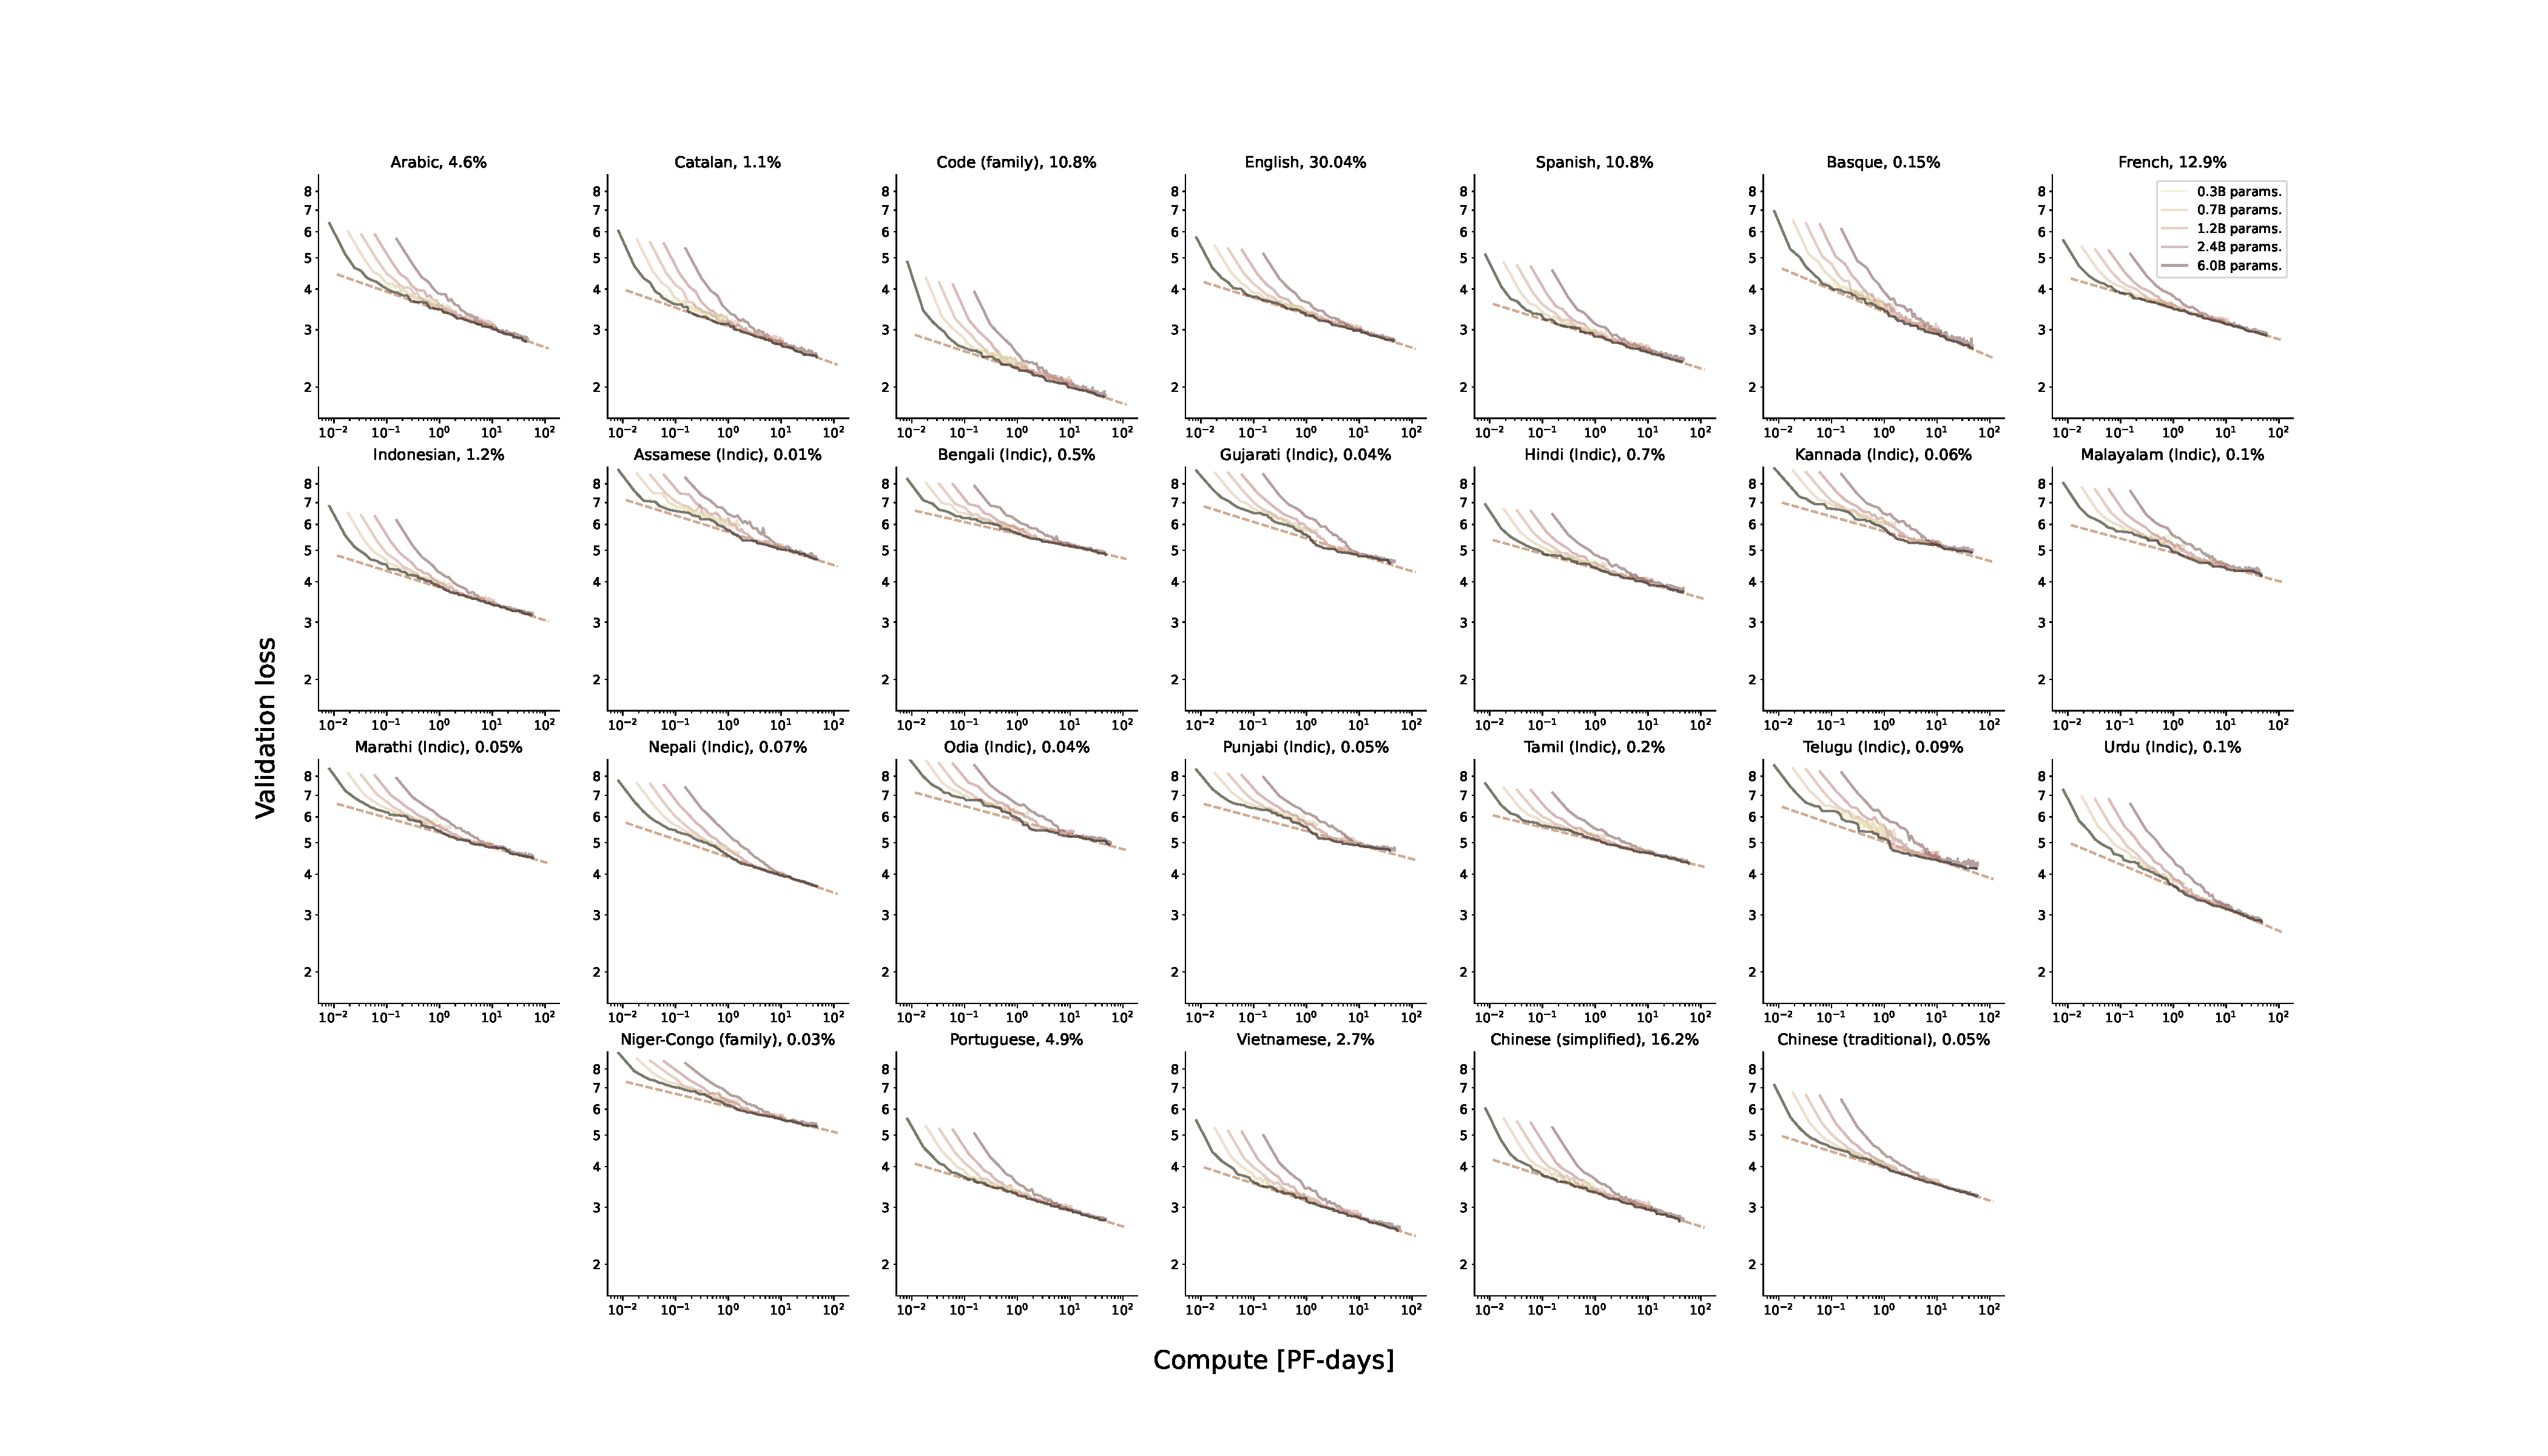
\includegraphics[width=1.1\textwidth]{figures/multilingual_scaling.pdf}}
    \caption{\textbf{Scaling laws across languages for the smaller BLOOM models}. Black line is Pareto frontier of optimality (best loss at a given compute), dashed line is best fit. Fit coefficients are detailed in Appendix \ref{sec:multilingualscalinglaws}. All sufficiently represented languages exhibit similar scaling behaviour, with mostly differences in loss offsets.}
    \label{fig:multilingualscaling}
\end{figure*}


\section{Scaling to 176B parameters}
We now detail how our previous findings influence our architecture and scaling decisions for the final 176B BLOOM model. % We have established that a curated high-quality cross-domain pretraining dataset similar to~\citet{gao2020pile} will help boost zero-shot generalization; adopted from \citet{wang2022language} that it is best to use a decoder-only model with an auto-regressive language modeling objective; identified that ALiBi positional embeddings should be used; and we have motivated the use of layer normalization on the embeddings to help with model stability. We should now determine which model architecture (e.g., number of parameters, layers, width) will result in the best model out of our compute budget. 

\paragraph{Compute allocation.} We have been allocated 18 weeks of dedicated use of partition with 52 nodes of 8x 80GB A100 GPUs on the Jean Zay supercomputer. We set four nodes aside as spare, so that our compute budget amounts to 1,161,216 A100-hours in total. Assuming a throughput of 100 model TFLOPS, approximately corresponding to state-of-the-art hardware FLOPS of 150~\cite{narayanan2021efficient}, we have a compute budget of 4,838 PF-days for the model training. We round this down to 4,500 PF-days, this $\sim10$\% safety margin accounting for potential downtime and inefficiencies (e.g., batch size ramp-up) during training. To put this number in perspective, this is $\sim23$\% more than the training budget of GPT-3. Given this compute budget, our English-only scaling laws in \ref{fig:scaling} predict an optimal allocation for training a 392B parameter model for 165B tokens. We will use these as an upper bound in size: the largest model we can afford is 392B parameters, and the minimum number of tokens to train on is 165B tokens.

% \subsection{Parameters, Tokens, and Shapes}
\begin{table*}[t]
\begin{small}
\begin{center}
\begin{tabular}{@{}lccccccc@{}}
\toprule
\multicolumn{1}{c}{\textbf{Model}} & \textbf{Size} & \textbf{Pretraining} & \textbf{Budget} & \textbf{Layers} & \textbf{Hidden dim.} & \multicolumn{2}{c}{\textbf{Attention heads}} \\ 
               & {[Bparams.]} & {[Btokens]}         & {[PF-days]}   &                 &                      & num.                  & dim.                 \\ \midrule
LaMDA \cite{thoppilan2022lamda}          & 137           & 432                  & 4,106            & 64              & 8,192                & 128                   & 64                   \\
GPT-3 \cite{brown2020gpt3}         & 175           & 300                  & 3,646            & 96              & 12,288               & 96                    & 128                  \\
J1-Jumbo \cite{J1WhitePaper}       & 178           & 300                  & 3,708            & 76              & 13,824               & 96                    & 144                  \\
PanGu-$\alpha$ \cite{zeng2021pangu} & 207           & 42                   & 604              & 64              & 16,384               & 128                   & 128                  \\
Yuan \cite{wu2021yuan}           & 245           & 180                  & 3,063            & 76              & 16,384               &  & \\
Gopher \cite{rae2021scaling}         & 280           & 300                  & 4,313            & 80              & 16,384               & 128                   & 128                  \\
MT-530B \cite{smith2022using}       & 530           & 270                  & 9,938            & 105             & 20,480               & 128                   & 160                  \\ \bottomrule
\end{tabular}
\end{center}
\end{small}
\caption{\textbf{State-of-the-art 100B+ models with publicly available details.} Compute budget is expressed in model PF-days required for training the models, from the $C= 6ND$ approximation of \citet{kaplan2020scaling}. Number of tokens for LaMDA is inferred from reported compute budget and size. Yuan did not report attention head details.}
\label{tab:sota_models}
\end{table*}

\begin{table*}[t]
\begin{small}
\begin{center}
\begin{tabular}{ccccccccc}
\toprule
\multicolumn{1}{c}{\textbf{Model}} & \textbf{Size} & \textbf{Layers} & \textbf{Hidden dim.}    & \multicolumn{2}{c}{\textbf{Attention heads}} & \multicolumn{1}{c}{\textbf{Memory}} & \multicolumn{2}{c}{\textbf{Performance}}                       \\
\multicolumn{1}{c}{}               & [params.]     &                 &                         & num.                  & dim.                 & \multicolumn{1}{c}{[GB]}            & \multicolumn{1}{c}{[sec/iter.]} & \multicolumn{1}{c}{[TFLOPs]} \\ \midrule
(1)                                & 178           & 82              & \multirow{2}{*}{13,312} & 64                    & 208                  & 63                                  & 104                             & 152                          \\
(2)                                & 178           & 82              &                         & 128                   & 104                  & 60                                  & 109                             & 146                          \\
\textbf{(3)}                                & \textbf{176}           & \textbf{70}              & \textbf{14,336}                  & \textbf{112}                   & \textbf{128}                  & \textbf{59}                                  & \textbf{105}                             & \textbf{150}                          \\ \bottomrule
\end{tabular}
\end{center}
\end{small}
\caption{\textbf{We choose configuration (3) as the final configuration for our 176B model.} (1) was rejected because of high attention heads dimension, and (3) was favored over (2) because of higher throughput. Appendix \ref{sec:arch_details} details all 20 final configurations benchmarked, only the best three are displayed here.}\label{tab:final_configs}
\end{table*}

% \paragraph{Fitting scaling laws.} 

%  We establish scaling laws~\cite{kaplan2020scaling} to verify the scaling behaviour of our model and codebase, and to help decide on optimal model size. 
% We use English data from OSCAR \citep{ortiz2019oscar} for pretraining, and train 125M, 350M, 760M, 1.3B, and 13B models for 100B to 300B tokens.  Figure~\ref{fig:scaling} shows the smooth decrease in loss against the compute budget as the model size increases. 

% We observe the following fit $L(C) = (C_c/C)^{\alpha_C}$ with $\alpha_C \approx 0.046$ and $C_c \approx 253 \times 10^8 \text{ PF-days}$. This scaling exponent $\alpha_C$ is inline with the 0.050 reported in \citet{kaplan2020scaling} and the 0.048 at larger scale in \citet{henighan2020scaling}. This is a remarkably close fit given that we are using different datasets, codebases, and hyperparameters. 

% One caveat is that these scaling coefficients are estimated on the OSCAR pretraining data, but we will apply them to the training of a multilingual model on a dataset that was not developed by the time these experiments were performed. Comparing the loss curves of the English and multilingual 1.3B models, we observe similar scaling and convergence trends. This suggests that the capacity of the model is the same whether it is trained on English or multilingual text. Therefore, we expect English-based scaling laws coefficients to still apply for a multilingual model. We additionally conjecture that they will transfer to our final dataset.


% \paragraph{Optimality vs. convergence.} From the scaling laws~\cite{kaplan2020scaling}, it is possible to derive a Pareto frontier describing the optimal allocation of the compute budget between model size and number of tokens seen. This optimal allocation achieves the lowest possible loss for a given compute budget. 
% It is notable that this Pareto optimal frontier describes large models trained on few tokens; we call this training to \emph{optimality}. This is in stark contrast with the common practice of training much smaller models on many more tokens to \emph{convergence}. For instance, for a 1.3B parameters model, \citet{kaplan2020scaling} predicts optimality at 20B tokens; any additional pretraining compute budget would be better allocated to a  larger model. 

% However, this only provides a partial view. Scaling laws focus on the upstream performance (pretraining loss) as the main evaluation metric, assuming that it directly translates to downstream performance. However, prior work showed that this is not always the case~\cite{Tay2021ScaleEI}. Additionally, Table~\ref{tab:validation} shows that zero-shot generalization continues improving significantly past optimality. 

% Scaling laws also neglect inference cost. A larger model is more expensive to serve, and inference costs at scale can catch up with training costs \cite{patterson2022carbon}. Finally, we note that most multilingual models are also trained for more tokens (e.g. XGLM on 500B tokens~\citet{XGLM}) than a similarly sized monolingual model, as the pretraining dataset will otherwise include very few tokens from low-resource languages.

% Accordingly, we choose to use the optimality front as an upper bound on model size and a lower bound on number of training tokens. Given our compute budget, scaling laws predict an optimal allocation for training a 392B parameter model for 165B tokens. Consequently, we will use these as constraints: the largest model we can afford is 392B parameters, and the minimum number of tokens to use is 165B tokens.

% \subsection{State-of-the-art models and recommendations}

% \paragraph{Prior models.} We outline in Table \ref{tab:sota_models} the architectures of all publicly detailed 100B+ parameters models at the time of this work. Most of these models are trained significantly beyond their respective optimality threshold, in the 300-400B tokens range. PanGu-$\alpha$ is the biggest exception, but this appears to be due to hardware availability constraints rather than actively motivated by a modeling decision. 

\paragraph{Model shape.} 
\citet{kaplan2020scaling} studied the dependence of the loss with model shape, and found only a limited impact within a wide range of feed-forward ratios $d_{ff} / d_{model}$, aspect ratios $d_{model}/n_{layer}$, and attention head dimensions. 

\citet{levine2020limits} proposed a theoretically motivated and empirically backed law describing the optimal compromise between width and depth. They predict that 100B+ parameters models such as GPT-3 are too deep, while models in the 10B or smaller range are usually too shallow. For a GPT-3-sized model with 175B parameters, they predict an ideal depth of 80 layers. 

\subsection{Final Model Architecture}

We set three main guidelines for our final model:
\begin{itemize}[leftmargin=*]
    \item \textbf{300-400B tokens.} 
    We want to guarantee our model will train on around 300-400B tokens of data. This is in the upper range for models in the size range we are pursuing, ensuring that low-resource languages will not be allocated too few tokens. Using the $C=6ND$ approximation \cite{kaplan2020scaling}, with $C=4,500$ PF-days and $D=300$-400B tokens, this constrains the model size to be around 160-200B parameters.
    \item \textbf{70-80 layers.} 
    From \citet{levine2020limits} and the size constraint above, we estimate that our model should have between 70 and 80 layers. 
    \item \textbf{Maximum throughput.}
    Finally, we want the final architecture to have as high of a throughput per GPU as possible, as more compute will translate directly into longer pretraining and thus a better model. Engineering constraints also come into light here: wide shallow models are typically easier to parallelize across nodes, up to a point where excessive tensor paralellism becomes necessary due to memory constraints.
\end{itemize}

We detail in Table \ref{tab:sota_models} the architectures of current state-of-the-art 100B+ models. From these guidelines, we benchmark 20 model configurations, detailed in Appendix~\ref{sec:arch_details}. Among these configurations, we select three of particular interest, outlined in Table~\ref{tab:final_configs}. They best fit our guidelines above, and offer high throughput, maximizing our training budget.

We discard configuration (1), as its attention heads are much larger than other models in the literature. Configuration (3) is shallower than recommended by \citet{levine2020limits}, but delivers 3\% higher throughput compared to (2). Thus, we choose configuration (3) and its better throughput, and because a shallower model is easier to deal with at inference time by introducing less latency. 


 
 
\section{Limitations}

\paragraph{Optimal scaling.} Concurrent to this work,  \citet{hoffmann2022training} identified more optimal scaling laws. For our compute budget, they would suggest a 50B parameters model trained for a trillion tokens. Interestingly, even in hindsight, it would have been difficult to follow this recommendation as we would have been limited by the limited availability of high-quality multilingual data and by the size of the BigScience training dataset, ROOTS \cite{roots}. Note that our Figure \ref{fig:scaling} reproduces \citet{kaplan2020scaling} as we did not account for the learning rate schedule as suggested by \citet{hoffmann2022training}.

\paragraph{Other hyperparameters.} 
In this work we have focused on a subset of the available hyperparameter space of large language models. We have investigated architecture decisions around positional embeddings, activation functions and the embedding norm. Alternative attention mechanisms \cite{tay2020long} or optimizers are examples of other dimensions that could be investigated, potentially leading to improved models.

\paragraph{Efficient fine-tuning.} 
Our study is focused on zero-shot use and does not consider efficient fine-tuning \cite{lester2021power, zaken2021bitfit}, which is quite relevant for large language models, and which may lead to different conclusions. 
 
\section{Conclusion}

% ======================================================================================== %
\section{Conclusion}\label{sec:conclusion}
% ======================================================================================== %

In this paper, we proposed a variant of self-attention (SA), named phonetic self-attention (phSA), to improve the ASR performance.
Especially, we investigated the phonetic behavior of attention heads and distinguished two different attention patterns, similarity-based and content-based attention.
The proposed phSA emphasized the two behaviors by applying simple and effective modifications to the original dot-product in SA.
In addition, the effect of each behavior is controlled by additional trainable parameters.
From the phoneme classification experiments, we showed that phSA is more suitable than the vanilla SA for phonetic feature extraction.
By replacing SA in lower layers with phSA, we improved the speech recognition performance on the end-to-end Transformer-based ASR model.
 
%\section*{Acknowledgements}

%\todo{Add acknowledgements.}

\bibliography{custom}
\bibliographystyle{acl_natbib}

\newpage


\appendix
\onecolumn

\section{Open artefacts: models, code, and logs}
\label{sec:artefacts}
We make public all artefacts produced as part of this work:
\begin{itemize}
    \item \textbf{Models.} All trained models are centralized at \url{https://huggingface.co/bigscience};
    \item \textbf{Code.} All code is available at \url{https://github.com/bigscience-workshop/Megatron-DeepSpeed/tree/main/megatron};
    \item \textbf{Discussions and logbook.} The notes from the weekly meetings of our working group are made available at \url{https://docs.google.com/document/d/1qbIkhd6bvbOsJOWXL7SfKQ0jey3MWQYQb_SshqH1LII/}.
\end{itemize}

\section{Multilingual scaling laws}
\label{sec:multilingualscalinglaws}

\begin{table*}[h]
\label{tab:multilingualscalinglaws}
\begin{center}
\begin{tabular}{cccc}
\toprule
Language & Proportion [\%] & $\alpha_c$ & $C_m$ \\
\midrule

Arabic & 4.6 & 0.057 & 1.16 \\
Catalan & 1.1 & 0.057 & 1.11\\
Code & 10.8 & 0.054 & 0.94\\
English & 30.0 & 0.051 & 1.08 \\
Spanish & 10.8 & 0.050 & 1.01 \\
Basque & 0.15 & 0.069 & 1.28 \\
French & 12.9 & 0.047 & 1.06\\
Indonesian & 1.2 & 0.051 & 1.14\\
Assamese & 0.01 & 0.051 & 1.31\\
Bengali & 0.5 & 0.037 & 1.15\\
Gujarati & 0.04 & 0.051 & 1.30\\
Hindi & 0.7 & 0.045 & 1.14\\
Kannada & 0.06 & 0.046 & 1.26\\
Malayalam & 0.1 & 0.044 & 1.17\\
Marathi & 0.05 & 0.046 & 1.23\\
Nepali & 0.07 & 0.055 & 1.25 \\
Odia & 0.04 & 0.044 & 1.25\\
Punjabi & 0.05 & 0.043 & 1.20\\
Tamil & 0.2 & 0.030 & 1.14\\
Telugu & 0.09 & 0.056 & 1.31\\
Urdu & 0.1 & 0.068 & 1.31\\
Niger-Congo (family) & 0.03 & 0.039 & 1.22\\
Portuguese & 4.9 & 0.049 & 1.05\\
Vietnamese & 2.7 & 0.053 & 1.08\\
Chinese (simplified) & 16.2 & 0.052 & 1.09\\
Chinese (traditionnal) & 0.05 & 0.050 & 1.15\\
\bottomrule

\end{tabular}
\caption{\textbf{Best scaling law fit per language.} We fit $\mathcal{L}(C) = C_m C^{-\alpha_c}$ to the runs reported in Figure \ref{fig:multilingualscaling}. But for a handful of languages which are poorly represented in the overall mixture (Basque, most of the Indic family, and Niger-Congo languages), scaling mostly different in offset $C_m$, not in exponent $\alpha_c$.}
\end{center}

\end{table*}

\newpage

\section{Evaluation details}
\label{sec:sup_eval}
\vfill
\begin{table*}[h]
\label{tab:sup_random-baselines}
\begin{center}
\begin{tiny}
\begin{tabular}{lllc}
\toprule
\multicolumn{2}{c}{\textbf{Task}} & \textbf{Type}           &  \textbf{Random baseline}                                \\ 
\midrule
ARC \citep{clark2018arc}      & Challenge & Natural Language Inference & 25.0       \\
             & Easy &     & 25.0                         \\
GLUE         & MRPC  \citep{dolan2016mrpc} & Paraphrase Identification      & 50.0                                                  \\
             & QQP \citep{iyer2019qqp} & Paraphrase Identification      & 50.0                                                             \\  
HellaSwag \citep{zellers2019hellaswag}    & & Sentence Completion           & 25.0                 \\
LAMBADA \citep{paperno2016lambada}      & & Sentence Completion       & 0.0                                        \\
LogiQA \citep{liu2020logiqa}      & & Multiple-Choice Question Answering           & 25.0                                               \\
MathQA \citep{amini2019mathqa}       & & Multiple-Choice Question Answering           & 20.1                                          \\
MC-TACO \citep{zhou2019mctaco} & & Multiple-Choice Question Answering & 36.2 \\
OpenBookQA \citep{mihaylov2press2021train018openbookqa}  & & Multiple-Choice Question Answering          & 25.0       \\
PIQA \citep{bisk2020piqa}         &  & Multiple-Choice Question Answering          & 50.0        \\
PROST  \citep{aroca-ouellette2021prost}        & & Multiple-Choice Question Answering          & 25.0                          \\
PudMedQA \citep{jin2019pubmedqa}     & & Multiple-Choice Question Answering          & 33.3                                         \\
QNLI \citep{rajpurkar2016squad,wang2019glue}         & & Sentence Completion           & 50.0                                         \\
Race \cite{lai2017large}        & & Closed-Book Question Answering         & 25.0                       \\
SciQ \citep{welbl2017sciq}         & & Multiple-Choice Question Answering          & 25.0                                          \\
SST \citep{socher2013sst}         & & Sentiment          & 50.0                                                \\
SuperGLUE    & Boolq \citep{clark2019boolq} & Multiple-Choice Question Answering     & 50.0                     \\
             & COPA \citep{gordon2012copa} & Sentence Completion      & 50.0 \\
             & MultiRC \citep{kashabi2018multirc} & Multiple-Choice Question Answering   & 5.8                                          \\
             & RTE \citep{dagan2005rte} & Natural Language Inference       & 50.0                     \\
             & WIC  \citep{pilehavar2018wic} & Word Sense Disambiguation       & 50.0                     \\
             & WSC \citep{levesque2012winograd} & Word Sense Disambiguation      & 50.0                     \\
TriviaQA \citep{joshi2017triviaqa}     & & Closed-Book Question Answering          & 0.0                      \\
WebQuestions \citep{berant2013semantic} & & Closed-Book Question Answering         & 0.0                        \\
Winogrande \citep{sakaguchi2019winogrande}   & & Coreference resolution           & 50.0             \\
WNLI \citep{sakaguchi2019winogrande}        & & Natural Language Inference         & 50.0      \\ \midrule
\textbf{EAI harness} & & & \textbf{33.3} \\
\bottomrule
\end{tabular}
\end{tiny}
\end{center}
\caption{\textbf{Evaluation tasks considered in the EAI harness and random baselines.}}
\vskip -0.1in
\end{table*}
\vfill
\newpage

\section{Architecture details}
\label{sec:arch_details}

\vfill

\begin{table}[h]
\vskip 0.15in
\begin{center}
\begin{small}
\centerline{\begin{tabular}{@{}cccccccccccc@{}}
\toprule
\multicolumn{5}{c}{\textbf{\sc{Architecture}}}                                                                                     & \multicolumn{4}{c}{\textbf{\sc{Parallelism}}}                                       & \multicolumn{3}{c}{\textbf{\sc{Performance}}}                \\ \midrule
\multicolumn{1}{l}{\textbf{Size}} & \textbf{Hidden dim.}    & \textbf{Layers}      & \multicolumn{2}{c}{\textbf{Attention heads}} & \textbf{Data}       & \textbf{Tensor}    & \textbf{Pipeline}   & \textbf{MBS}       & \textbf{Memory}    & \multicolumn{2}{c}{\textbf{Throughput}} \\
 {[Bparams.]}                      &                         &                      & num.                 & dim.                  &                     &                    &                     &                    & [GB]               & [s/iter.]            & [TFLOPs]           \\ \midrule
206                               & 14,336                  & 82                   & 128                  & 112                   & 8                   & 4                  & 12                  & 2                  & \ul{OOM}           &                      &                  \\ \midrule
203                               & 13,312                  & 94                   & 128                  & 104                   & 8                   & 4                  & 12                  & 2                  & 67                 & 124,1                & 146,1            \\ \midrule 
\multirow{4}{*}{195}              & \multirow{4}{*}{12,288} & \multirow{4}{*}{106} & 128                  & 96                    & \multirow{4}{*}{8}  & \multirow{4}{*}{4} & \multirow{4}{*}{12} & 2                  & 67                 & 121,4                & 143,7            \\
                                  &                         &                      & \multirow{2}{*}{96}  & 128                   &                     &                    &                     & 4                  & 79                 & 120,3                & 145,0            \\
                                  &                         &                      &                      & 128                   &                     &                    &                     & \multirow{2}{*}{2} & 65                 & 118,8                & 146,9            \\
                                  &                         &                      & 64                   & 192                   &                     &                    &                     &                    & 67                 & 116,5                & 149,8            \\\midrule
\multirow{4}{*}{184}              & \multirow{4}{*}{12,288} & \multirow{4}{*}{100} & \multirow{4}{*}{64}  & \multirow{4}{*}{192}  & \multirow{2}{*}{16} & \multirow{2}{*}{4} & \multirow{4}{*}{6}  & 2                  & \ul{OOM}           &                      &                  \\
                                  &                         &                      &                      &                       &                     &                    &                     & 1                  & \ul{OOM}           &                      &                  \\
                                  &                         &                      &                      &                       & \multirow{2}{*}{8}  & \multirow{2}{*}{8} &                     & 4                  & 72                 & 121,0                & 136,2            \\
                                  &                         &                      &                      &                       &                     &                    &                     & 2                  & 61                 & 140,0                & 117,9            \\\midrule
\multirow{5}{*}{178}              & \multirow{5}{*}{13,312} & \multirow{5}{*}{82}  & 128                  & 104                   & \multirow{3}{*}{8}  & \multirow{3}{*}{4} & \multirow{5}{*}{12} & \multirow{2}{*}{2} & 60                 & 108,8                & 145,7            \\
                                  &                         &                      & 104                  & 128                   &                     &                    &                     &                    & 62                 & 123,7                & 128,1            \\
                                  &                         &                      & \multirow{3}{*}{64}  & \multirow{3}{*}{208}  &                     &                    &                     & \multirow{2}{*}{4} & 74                 & 104,8                & 151,2            \\
                                  &                         &                      &                      &                       & 4                   & 8                  &                     &                    & 52                 & 111,8                & 141,8            \\
                                  &                         &                      &                      &                       & 8                   & 4                  &                     & 2                  & 63                 & 104,5                & 151,7            \\\midrule
\multirow{5}{*}{176}              & \multirow{5}{*}{14,336} & \multirow{5}{*}{70}  & 128                  & 112                   & \multirow{4}{*}{8}  & \multirow{4}{*}{4} & \multirow{4}{*}{12} & \multirow{2}{*}{2} & 60                 & 105,9                & 148,1            \\
                                  &                         &                      & 112                  & 128                   &                     &                    &                     &                    & 59                 & 104,5                & 150,1            \\
                                  &                         &                      & \multirow{3}{*}{64}  & \multirow{3}{*}{224}  &                     &                    &                     & 4                  & 73                 & 102,3                & 153,3            \\
                                  &                         &                      &                      &                       &                     &                    &                     & \multirow{2}{*}{2} & 59                 & 102,0                & 153,7            \\
                                  &                         &                      &                      &                       & 4                   & 8                  & 12                  &                    & 40                 & 121,6                & 128,9            \\ \bottomrule

\end{tabular}}
\end{small}
\end{center}
\caption{\textbf{Throughput and memory usage of considered models sizes.} Note that pipeline parallelism here considers equal "slots" for embeddings and Transformer layers. This is important to optimize pipeline use, as our multilingual embeddings are quite large (250k).}
\label{tab:sup_throughput}
\end{table}

\vfill


\newpage
\section{All Results}
\label{sec:all_results}

\begin{table}[h]
\vskip 0.15in
\begin{center}
\begin{small}
\centerline{\begin{tabular}{lllllllll}
\toprule
Ablation       & Dataset  & Embedding & Activation & Embedding Norm & Parameters & 112GT   & 250GT   & 300GT   \\ \midrule
Embeddings     & OSCAR    & Learned   & GELU       & No             & 1.3B       & 41.71 &       &       \\
Embeddings     & OSCAR    & None      & GELU       & No             & 1.3B       & 41.23 &       &       \\
Embeddings     & OSCAR    & Rotary    & GELU       & No             & 1.3B       & 41.46 &       &       \\
Embeddings     & OSCAR    & ALiBi     & GELU       & No             & 1.3B       & 43.70 &       &       \\\midrule
Dataset        & The Pile & Learned   & GELU       & No             & 1.3B       & 42.79 & 43.12 & 43.46 \\
Dataset        & C4       & Learned   & GELU       & No             & 1.3B       & 42.77 &       &       \\
Dataset        & OSCAR    & Learned   & GELU       & No             & 1.3B       & 42.79 &       &       \\\midrule
Activation     & The Pile & Learned   & GELU       & No             & 1.3B       & 42.79 &       &       \\
Activation     & The Pile & Learned   & SwiGLU     & No             & 1.3B       & 42.95 &       &       \\\midrule
Embedding Norm & The Pile & Learned   & GELU       & No             & 1.3B       & 42.79 & 43.12 & 43.46 \\
Embedding Norm & The Pile & Learned   & GELU       & Yes            & 1.3B       &       &       & 42.24 \\\midrule
Multilinguality             & OSCAR-ML & Learned   & GELU       & No             & 1.3B       & 38.55 &       &       \\
Multilinguality             & OSCAR    & Learned   & GELU       & No             & 1.3B       & 41.72 &       &       \\\midrule
Scale           & OSCAR    & Learned   & GELU       & No             & 1.3B       & 41.72 &       &       \\
Scale           & OSCAR    & Learned   & GELU       & No             & 13B        &       &       & 47.09\\
\bottomrule
\end{tabular}}
\end{small}
\end{center}
\caption{\textbf{Summary of all results obtained in this study}. The final three columns indicate the average EAI Harness results at across different billion tokens trained. Some rows are duplicated for ease of reading.}

\label{tab:all_results}
\end{table}






\begin{sidewaystable}
\centering
\begin{tiny}
\begin{tabular}{lllllllllllllllllll}
Public Name                 & ~         & ~                       & OpenAI:
  babbage & Openai:
  curie & gpt-neo
  1.3B & ~       & ~       & ~        & ~        & ~        & ~        & ~        & ~       & ~        & ~       & ~       & ~       & ~         \\
Dataset                     & ~         & ~                       & ~                 & ~               & ~              & C4      & OSCAR   & The Pile & The Pile & The Pile & The Pile & The Pile & OSCAR   & The Pile & OSCAR   & OSCAR   & OSCAR   & OSCAR-ML  \\
Embeddings                  & ~         & ~                       & ~                 & ~               & ~              & Learned & Learned & Learned  & Learned  & Learned  & Learned  & Learned  & Learned & Learned  & Rotary  & ALiBi   & None    & Learned   \\
Activation                  & ~         & ~                       & ~                 & ~               & ~              & GELU    & GELU    & GELU     & GELU     & GELU     & GELU     & GELU     & GELU    & SwiGLU   & GELU    & GELU    & GELU    & GELU      \\
Embedding Norm              & ~         & ~                       & ~                 & ~               & ~              & No      & No      & No       & No       & No       & No       & No       & No      & No       & No      & No      & No      & No        \\
Parameters in billion                 & ~         & ~                       & 1.3               & 6.7             & 1.3            & 1.3     & 1.3     & 1.3      & 1.3      & 1.3      & 1.3      & 1.3      & 13     & 1.3      & 1.3     & 1.3     & 1.3       & 1.3       \\
Tokens
  trained in billion & ~         & ~                       & 300               & 300             & 300            & 112     & 112     & 112      & 250      & 300      & 300      & 330      & 300     & 112      & 112     & 112     & 112     & 112       \\
task                        & metric    & ~                       & ~                 & ~               & ~              & ~       & ~       & ~        & ~        & ~        & ~        & ~        & ~       & ~        & ~       & ~       & ~       & ~         \\
arc\_challenge              & acc       & arc\_challengeacc       & 0.276             & 0.334           & 0.231          & 0.243   & 0.249   & 0.258    & 0.264    & 0.260    & 0.242    & 0.250    & 0.322   & 0.247    & 0.236   & 0.252   & 0.249   & 0.212     \\
arc\_challenge              & acc\_norm & arc\_challengeacc\_norm & 0.295             & 0.375           & 0.259          & 0.274   & 0.261   & 0.275    & 0.277    & 0.286    & 0.277    & 0.290    & 0.342   & 0.268    & 0.270   & 0.276   & 0.260   & 0.243     \\
arc\_easy                   & acc       & arc\_easyacc            & 0.597             & 0.685           & 0.562          & 0.561   & 0.560   & 0.556    & 0.569    & 0.601    & 0.568    & 0.582    & 0.681   & 0.557    & 0.554   & 0.575   & 0.537   & 0.484     \\
arc\_easy                   & acc\_norm & arc\_easyacc\_norm      & 0.555             & 0.633           & 0.502          & 0.503   & 0.478   & 0.506    & 0.518    & 0.528    & 0.516    & 0.515    & 0.600   & 0.502    & 0.476   & 0.491   & 0.461   & 0.434     \\
boolq                       & acc       & boolqacc                & 0.629             & 0.666           & 0.620          & 0.546   & 0.566   & 0.520    & 0.551    & 0.606    & 0.558    & 0.566    & 0.587   & 0.540    & 0.584   & 0.563   & 0.526   & 0.597     \\
copa                        & acc       & copaacc                 & 0.810             & 0.850           & 0.690          & 0.700   & 0.720   & 0.710    & 0.710    & 0.730    & 0.690    & 0.690    & 0.880   & 0.660    & 0.690   & 0.780   & 0.680   & 0.710     \\
hellaswag                   & acc       & hellaswagacc            & 0.429             & 0.504           & 0.387          & 0.422   & 0.404   & 0.374    & 0.385    & 0.405    & 0.378    & 0.380    & 0.542   & 0.379    & 0.410   & 0.422   & 0.395   & 0.340     \\
hellaswag                   & acc\_norm & hellaswagacc\_norm      & 0.545             & 0.664           & 0.489          & 0.551   & 0.515   & 0.464    & 0.486    & 0.521    & 0.477    & 0.476    & 0.716   & 0.475    & 0.524   & 0.549   & 0.495   & 0.424     \\
lambada                     & acc       & lambadaacc              & 0.625             & 0.694           & 0.572          & 0.469   & 0.481   & 0.569    & 0.575    & 0.609    & 0.581    & 0.580    & 0.634   & 0.574    & 0.496   & 0.501   & 0.454   & 0.408     \\
logiqa                      & acc       & logiqaacc               & 0.201             & 0.215           & 0.197          & 0.206   & 0.237   & 0.210    & 0.218    & 0.203    & 0.217    & 0.223    & 0.232   & 0.215    & 0.210   & 0.215   & 0.237   & 0.218     \\
logiqa                      & acc\_norm & logiqaacc\_norm         & 0.269             & 0.292           & 0.273          & 0.267   & 0.270   & 0.275    & 0.286    & 0.269    & 0.281    & 0.280    & 0.275   & 0.272    & 0.254   & 0.272   & 0.293   & 0.283     \\
mathqa                      & acc       & mathqaacc               & 0.244             & 0.251           & 0.241          & 0.233   & 0.222   & 0.249    & 0.248    & 0.263    & 0.246    & 0.245    & 0.238   & 0.245    & 0.234   & 0.237   & 0.215   & 0.223     \\
mathqa                      & acc\_norm & mathqaacc\_norm         & 0.242             & 0.247           & 0.237          & 0.228   & 0.228   & 0.246    & 0.245    & 0.259    & 0.242    & 0.242    & 0.235   & 0.234    & 0.229   & 0.238   & 0.221   & 0.222     \\
mc\_taco                    & f1        & mc\_tacof1              & 0.458             & 0.484           & 0.493          & 0.361   & 0.293   & 0.485    & 0.488    & 0.494    & 0.487    & 0.489    & 0.497   & 0.493    & 0.461   & 0.337   & 0.477   & 0.387     \\
mrpc                        & acc       & mrpcacc                 & 0.578             & 0.684           & 0.684          & 0.684   & 0.588   & 0.684    & 0.684    & 0.684    & 0.679    & 0.679    & 0.677   & 0.684    & 0.684   & 0.684   & 0.679   & 0.302     \\
mrpc                        & f1        & mrpcf1                  & 0.718             & 0.812           & 0.812          & 0.812   & 0.702   & 0.812    & 0.812    & 0.812    & 0.808    & 0.809    & 0.806   & 0.812    & 0.812   & 0.812   & 0.808   & 0.090     \\
multirc                     & acc       & multircacc              & 0.018             & 0.015           & 0.018          & 0.018   & 0.026   & 0.023    & 0.024    & 0.023    & 0.025    & 0.008    & 0.018   & 0.026    & 0.009   & 0.011   & 0.016   & 0.040     \\
openbookqa                  & acc       & openbookqaacc           & 0.224             & 0.290           & 0.216          & 0.220   & 0.200   & 0.190    & 0.196    & 0.222    & 0.194    & 0.208    & 0.294   & 0.214    & 0.212   & 0.224   & 0.210   & 0.170     \\
openbookqa                  & acc\_norm & openbookqaacc\_norm     & 0.336             & 0.386           & 0.336          & 0.336   & 0.328   & 0.316    & 0.314    & 0.334    & 0.302    & 0.312    & 0.412   & 0.320    & 0.344   & 0.340   & 0.332   & 0.276     \\
piqa                        & acc       & piqaacc                 & 0.745             & 0.763           & 0.711          & 0.732   & 0.716   & 0.693    & 0.704    & 0.716    & 0.698    & 0.706    & 0.777   & 0.693    & 0.720   & 0.729   & 0.711   & 0.674     \\
piqa                        & acc\_norm & piqaacc\_norm           & 0.746             & 0.772           & 0.711          & 0.730   & 0.721   & 0.705    & 0.705    & 0.717    & 0.698    & 0.701    & 0.788   & 0.689    & 0.721   & 0.731   & 0.711   & 0.682     \\
prost                       & acc       & prostacc                & 0.270             & 0.288           & 0.238          & 0.243   & 0.237   & 0.249    & 0.229    & 0.204    & 0.219    & 0.226    & 0.281   & 0.244    & 0.287   & 0.280   & 0.240   & 0.253     \\
prost                       & acc\_norm & prostacc\_norm          & 0.260             & 0.295           & 0.308          & 0.293   & 0.303   & 0.268    & 0.271    & 0.268    & 0.292    & 0.305    & 0.283   & 0.276    & 0.296   & 0.332   & 0.300   & 0.313     \\
pubmedqa                    & acc       & pubmedqaacc             & 0.611             & 0.622           & 0.544          & 0.573   & 0.438   & 0.563    & 0.589    & 0.662    & 0.612    & 0.612    & 0.615   & 0.589    & 0.507   & 0.514   & 0.486   & 0.412     \\
qnli                        & acc       & qnliacc                 & 0.512             & 0.529           & 0.499          & 0.476   & 0.507   & 0.505    & 0.506    & 0.505    & 0.499    & 0.499    & 0.517   & 0.498    & 0.493   & 0.481   & 0.493   & 0.493     \\
qqp                         & acc       & qqpacc                  & 0.372             & 0.441           & 0.382          & 0.396   & 0.384   & 0.381    & 0.370    & 0.375    & 0.371    & 0.369    & 0.368   & 0.435    & 0.370   & 0.423   & 0.370   & 0.389     \\
qqp                         & f1        & qqpf1                   & 0.534             & 0.515           & 0.522          & 0.530   & 0.519   & 0.534    & 0.537    & 0.537    & 0.538    & 0.538    & 0.533   & 0.495    & 0.539   & 0.475   & 0.537   & 0.505     \\
race                        & acc       & raceacc                 & 0.356             & 0.386           & 0.341          & 0.330   & 0.323   & 0.334    & 0.329    & 0.344    & 0.321    & 0.323    & 0.374   & 0.337    & 0.317   & 0.344   & 0.332   & 0.326     \\
rte                         & acc       & rteacc                  & 0.585             & 0.552           & 0.603          & 0.502   & 0.534   & 0.563    & 0.549    & 0.578    & 0.563    & 0.549    & 0.524   & 0.527    & 0.545   & 0.524   & 0.527   & 0.505     \\
sciq                        & acc       & sciqacc                 & 0.867             & 0.919           & 0.860          & 0.825   & 0.810   & 0.838    & 0.853    & 0.868    & 0.860    & 0.867    & 0.895   & 0.849    & 0.818   & 0.828   & 0.816   & 0.793     \\
sciq                        & acc\_norm & sciqacc\_norm           & 0.809             & 0.896           & 0.770          & 0.747   & 0.717   & 0.755    & 0.762    & 0.792    & 0.791    & 0.803    & 0.815   & 0.770    & 0.718   & 0.728   & 0.698   & 0.702     \\
sst                         & acc       & sstacc                  & 0.732             & 0.666           & 0.656          & 0.676   & 0.560   & 0.753    & 0.721    & 0.501    & 0.528    & 0.710    & 0.514   & 0.760    & 0.493   & 0.588   & 0.588   & 0.510     \\
triviaqa                    & acc       & triviaqaacc             & 0.115             & 0.195           & 0.052          & 0.027   & 0.025   & 0.056    & 0.065    & 0.058    & 0.047    & 0.049    & 0.133   & 0.050    & 0.031   & 0.039   & 0.028   & 0.021     \\
webqs                       & acc       & webqsacc                & 0.048             & 0.065           & 0.017          & 0.012   & 0.004   & 0.023    & 0.026    & 0.023    & 0.020    & 0.021    & 0.027   & 0.012    & 0.006   & 0.004   & 0.015   & 0.001     \\
wic                         & acc       & wicacc                  & 0.495             & 0.500           & 0.500          & 0.495   & 0.508   & 0.495    & 0.500    & 0.500    & 0.498    & 0.500    & 0.498   & 0.500    & 0.498   & 0.492   & 0.500   & 0.500     \\
winogrande                  & acc       & winograndeacc           & 0.595             & 0.648           & 0.551          & 0.564   & 0.565   & 0.536    & 0.552    & 0.560    & 0.533    & 0.543    & 0.647   & 0.538    & 0.564   & 0.583   & 0.543   & 0.519     \\
wsc                         & acc       & wscacc                  & 0.394             & 0.558           & 0.365          & 0.539   & 0.567   & 0.365    & 0.365    & 0.365    & 0.414    & 0.385    & 0.500   & 0.365    & 0.394   & 0.635   & 0.462   & 0.539     \\
Avg
  acc                   & ~         & ~                       & 45.30\%           & 49.28\%         & 42.94\%        & 42.77\% & 41.72\% & 42.79\%  & 43.12\%  & 43.46\%  & 42.24\%  & 43.08\%  & 47.09\% & 42.95\%  & 41.45\% & 43.70\% & 41.23\% & 38.55\%  
\end{tabular}
\end{tiny}
\end{sidewaystable}


\end{document}